%------------------------------------
% To be edited
%------------------------------------
\newcommand{\documentname}{Floating point CORDIC de doble precisi\'on}
\newcommand{\crev}{0.5}
\newcommand{\documentversion}{Rev. \crev}
\newcommand{\cryear}{2016}
\hyphenation{soft-ware hard-ware}
%------------------------------------

\documentclass[10pt,a4paper]{book}
\setlength{\parindent}{0pt}
\setlength{\parskip}{1ex plus 0.5ex minus 0.2ex}
\addtolength{\headsep}{0.5cm}
\usepackage[a4paper]{geometry} %,left=2.5cm,right=3.5cm
\usepackage[colorlinks=false]{hyperref}
\usepackage[english, activeacute]{babel}
\usepackage[utf8]{inputenc}
\usepackage{graphics}
\usepackage[final]{graphicx}
\usepackage{caption}
\usepackage{subcaption}
\usepackage{float}                        %  alows using subfloat for graphics
\usepackage[maxfloats=256]{morefloats}    %  max number of floating figures ( in the appendices you have like 200)
\usepackage{rotating}
\usepackage{color}
\usepackage{longtable}
\usepackage{latexsym}
\usepackage{multicol}
\usepackage{multirow}
\usepackage{fancyhdr}
\usepackage{gensymb}                      % for degree symbol
\usepackage{listings}                     % to show source code
\lstloadlanguages{VHDL}
\usepackage{tikz}                         % for DIA graphics
\usepackage{makeidx}                      % to make the index
%%%%%%%%%\usepackage{bytefield}

% Paquetes matematicos
\usepackage{amsfonts}
\usepackage{amsmath}
\usepackage{amssymb}
\usepackage{amsthm}
\usepackage{mathrsfs}
\DeclareMathOperator\arctanh{arctanh}

\pagestyle{fancy}

%\usepackage{anysize}
%\marginsize{3cm}{4cm}{2.5cm}{3.5cm}

%---- Encabezado y pie de pagina general
\fancypagestyle{general}
{
   \fancyhf{}
   \fancyfoot{}
   \fancyhead{}
   \fancyhead[LO]{\footnotesize{\leftmark}}
   \fancyhead[RE]{\footnotesize{\rightmark}}
   \fancyhead[RO]{\footnotesize{\thepage}}
   \fancyhead[LE]{\footnotesize{\thepage}}
   \renewcommand{\headrulewidth}{0pt}
   \renewcommand{\footrulewidth}{0pt}
   }

\fancypagestyle{plain}
{
   \fancyhf{}
   \fancyfoot{}
   \fancyhead{}
   \fancyfoot[RO]{\footnotesize{\thepage}}
   \fancyfoot[LE]{\footnotesize{\thepage}}
   \renewcommand{\headrulewidth}{0pt}
   \renewcommand{\footrulewidth}{0pt}
   }

%---- Encabezado y pie de pagina de la caratula
\fancypagestyle{carat} {
   \fancyhf{}
   \fancyfoot{}
   \fancyhead{}
   \fancyhead[LO]{\scalebox{0.15}{
\includegraphics[angle=0]{./figures/logo_lab_ue_3.png}}}
   \fancyhead[RE]{}
   \fancyhead[RO]{\scalebox{0.5}{
\includegraphics[angle=0]{./figures/logo_fiuba.jpg}}}
   \fancyhead[LE]{}
   \fancyhead[CE]{}
   \fancyfoot[CO]{\textcircled{c} Lab-$\mu$E, FIUBA. \cryear.}
   \renewcommand{\headrulewidth}{0pt}
   \renewcommand{\footrulewidth}{1pt}
}

%---- Quito los encabezados y pies de pagina en las hojas vacias
\makeatletter
  \def\cleardoublepage{\clearpage\if@twoside \ifodd\c@page\else
  \vspace*{\fill}
    \thispagestyle{empty}
    \newpage
    \if@twocolumn\hbox{}\newpage\fi\fi\fi}
\makeatother

%---- Espaciado en el indice entre el numero y el titulo
\makeatletter
\renewcommand*{\l@subsection}{\@dottedtocline{1}{3.8em}{3.5em}}
\renewcommand*{\l@figure}{\@dottedtocline{1}{1.5em}{3.3em}}
\renewcommand*{\l@table}{\@dottedtocline{1}{1.5em}{2.8em}}
\makeatother

%---- Formateo del codigo VHDL
\lstset
{
   %extendedchars=true,%
   %labelstep=0,
   %labelsep=3ex,
   %frame=trbl,
   %frameround=tttt,
   %framespread=-3ex,
   %framerulecolor=colorFondoListado,
   %backgroundcolor=colorFondoListado,
   captionpos=b,
   breaklines=true,
   %linewidth=0.98\linewidth,
   %indent=5ex,
   tabsize=4,
   %labelstyle=\small\ttfamily,
   basicstyle=\scriptsize\sffamily,
   %numberstyle=\small\sffamily,
   identifierstyle=\scriptsize\sffamily,
   commentstyle=\scriptsize\itshape,
   stringstyle=\scriptsize\sffamily,
   keywordstyle=\scriptsize\bfseries\sffamily,
   ndkeywordstyle=\scriptsize\bfseries\sffamily,
   showstringspaces=false,
   flexiblecolumns=false
   visiblespaces=false
   %stringspaces=false
}

%---- Encabezado y pie de pagina por defecto
\pagestyle{general}

%---- Matematica
\newtheorem{defi}{Definici\'on}
\newtheorem{teor}{Teorema}
\newtheorem{prop}{Proposici\'on}
\newtheorem{lema}{Lema}
\newtheorem{cor}{Corolario}
\DeclareMathOperator{\sen}{sen}
\DeclareMathOperator{\supr}{sup}
\DeclareMathOperator{\sgn}{sgn}
\DeclareMathOperator{\lip}{lip}
\DeclareMathOperator{\codim}{codim}
\DeclareMathOperator{\gen}{gen}
\DeclareMathOperator{\im}{Im}
\DeclareMathOperator{\nuc}{Nu}
\DeclareMathOperator{\ind}{ind}
\DeclareMathOperator{\dom}{Dom}
\DeclareMathOperator{\real}{Real}
\DeclareMathOperator{\imag}{Imag}

%---- Para no separar en SILABAS se activa el comando siguiente
\hyphenpenalty=10000


\begin{document}

%------------------------------------------------
% 1.Introducción
%------------------------------------------------
\chapter{CORDIC}

% 1.1 Algoritmo CORDIC
\section{Algoritmo CORDIC}

El algoritmo CORDIC propuesto por Volder realizaba rotaciones en coordenadas circulares.
Partiendo de esa base es facil extender su funcionamiento para que realice rotaciones en coordenadas hiperbólicas y lineales. Para lograrlo se agrega una variables que modifica las ecuaciones y además se eligen diferentes angulos para el acumulador de angule (variable z del algoritmo).
Las ecuaciones del CORDIC completo son:
\begin{equation} \label{eq:cordic_eq}
   \begin{subequations}
      \begin{aligned}
         x_{n+1} &=  x_n - m \cdot d_n \cdot 2^{-s_{m,n}}   \\
         y_{n+1} &=  y_n + d_n \cdot 2^{-s_{m,n}}             \\
         z_{n+1} &=  z_n - d_n \cdot \alpha_{m,n}
      \end{aligned}
   \end{subequations}
\end{equation}

Donde $N$ representa la cantidad de pasos del algoritmo y se cumple que $n= 0, 1, 2, ... , N-1$. $s_{m,n}$ es una sequencia de números enteros no decreciente llamada \textit{shift sequence} y $\alpha_{m,n}$ representa los angulos rotados para las diferentes coordenadas. $d_n$ es una variable de control que maneja los sumadores/restadores.
\begin{equation} \label{eq:rotation_angle}
   \alpha_{m,n} = \dfrac {1}{\sqrt{m}} \cdot \tan^{-1}(\sqrt{m} \cdot 2^{-s_{m,n}} )
\end{equation}

Eligiendo correctamente $d_n$ y $s_{m,n}$ el algoritmo converge (ver tabla ~\ref{tab:table_shift_seq}). La tabla ~\ref{tab:table_cordic_outputs} muestra las diferentes salidas del algoritmo. En la table ~\ref{tab:table_cordic_outputs_special_cases} podemos ver las salidas del algoritmo para valores de entrada particulares, estos valores son de especial interés ya que representan operaciones matematicas difíciles de calcular.

\begin{table}[h!]
\centering
\begin{tabular}{llll}
   \hline
   Sistema de coordenadas  &  Shift sequence       &  Convergencia   &  Factor de escala                 \\ \hline \hline
   $m$                     &  $s_{m,n}$            &  $|A_0|$        &  $K_{m} (n \rightarrow \inf)$     \\ \hline
   1                       &  0,1,2, ... , n       &  $ 1.74$        &  $1.64676$                        \\ \hline
   0                       &  1,2,3, ... , n+1     &  $ 1.0 $        &  $1.0    $                        \\ \hline
   -1                      &  1,2,3,4,4, ...       &  $ 1.13$        &  $0.82816$                        \\ \hline \hline
\end{tabular}
\caption{CORDIC shift sequences}
\label{tab:table_shift_seq}
\end{table}

\begin{table}[h!]
\centering
\begin{tabular}{clll}
   \hline
   $m$   &  Modo     &  Entradas          & Salidas                                                \\ \hline \hline
   1     &  rotation &  $x_0 = x$         & $x_N = K_1 \cdot (x \cos\theta - y \sin\theta)$        \\
         &           &  $y_0 = y$         & $y_N = K_1 \cdot (y \cos\theta + x \sin\theta)$        \\
         &           &  $z_0 = \theta$    & $z_N = 0$                                              \\ \hline
   1     &  vectoring&  $x_0 = x$         & $x_N = K_1 \cdot sign(x) \cdot \sqrt{x^2+y^2}$         \\
         &           &  $y_0 = y$         & $y_N = 0$                                              \\
         &           &  $z_0 = \theta$    & $z_N = \theta + \tan^{-1}(y/x)$                        \\ \hline
   0     &  rotation &  $x_0 = x$         & $x_N = x $                                             \\
         &           &  $y_0 = y$         & $y_N = y + x \cdot z$                                  \\
         &           &  $z_0 = \theta$    & $z_N = 0$                                              \\ \hline
   0     &  vectoring&  $x_0 = x$         & $x_N = x$                                              \\
         &           &  $y_0 = y$         & $y_N = 0$                                              \\
         &           &  $z_0 = z$         & $z_N = z + y / x$                                      \\ \hline
   -1    &  rotation &  $x_0 = x$         & $x_N = K_{-1} \cdot (x \cosh\theta + y \sinh\theta)$   \\
         &           &  $y_0 = y$         & $y_N = K_{-1} \cdot (y \cosh\theta + x \sinh\theta)$   \\
         &           &  $z_0 = \theta$    & $z_N = 0$                                              \\ \hline
   -1    &  vectoring&  $x_0 = x$         & $x_N = K_{-1} \cdot sign(x) \cdot \sqrt{x^2-y^2}$      \\
         &           &  $y_0 = y$         & $y_N = 0$                                              \\
         &           &  $z_0 = \theta$    & $z_N = \theta + \tanh^{-1}(y/x)$                       \\ \hline
\end{tabular}
\caption{Salidas del algoritmo CORDIC.}
\label{tab:table_cordic_outputs}
\end{table}


\chapter{Algoritmo de Briggs para ln(x)}

Si se encuentra una secuencia $d_k$ tal que la productoria de $x$ con $(1+d_k 2^{-k})$ es cercana a 1 entonces vale que:

\begin{equation} \label{eq:briggs_ln}
   \begin{subequations}
      \begin{aligned}
         x \prod_{k=1}^{n} (1+d_k 2^{-k}) \approx 1     \\
         ln(x) \approx - \sum_{k=1}^{n} \ln(1+d_k 2^{-k})
      \end{aligned}
   \end{subequations}
\end{equation}


\chapter{BKM}

   \section{El algoritmo}
   \subsection{Origenes}

   Consideremos el paso básico del algoritmo CORDIC en modo trigonométrico (con m=1).
   Si definimos el número complejo $E_n = x_n + j \, y_n$ con $j=\sqrt{-1}$, obtenemos $E_{n+1} = E_n (1+j \, d_n 2^{-n})$, esta relación es similar al paso básico del algorithmo de Briggs.
   Esta similitud nos lleva a una generalización de ese algoritmo: podriamos realizar multiplicaciones por terminos $(1+d_n 2^{-n})$, donde los $d_n$s son números complejos elejidos de tal manera que la multiplicación por $d_n$ pueda reducirce a unas pocas sumas.
   Entonces se define el algoritmo BKM de la siguiente manera:

\begin{equation} \label{eq:bkm_eqs}
   \left\{
      \begin{aligned}
         E_{n+1} &= E_n \cdot (1 + d_n 2^{-n})   \\
         L_{n+1} &= L_n - \ln(1 + d_n 2^{-n})
      \end{aligned}
   \right.
\end{equation}

   con $d_n = d_n^r + j d_n^i $ y $d_n^r, d_n^i \in \{ 0, \pm 1 \}$ y $\ln z = t$ es el número complejo $t$ tal que $\exp{t} = z$ y cuya parte imaginaria está entre $-\pi$ y $\pi$.


   \subsection{N\'umero de constantes}

   Este algoritmo requiere que se almacenen las constantes referidas a $\ln(1 + d_n 2^{-n})$.

   \begin{equation} \label{eq:bkm_constants}
      \left\{
         \begin{aligned}
            \Re \{\ln(1 + d_n 2^{-n})\} &= \frac{1}{2} \ln[ 1 + d_n^r \, 2^{-n+1} + ({d_n^r}^2 + {d_n^i}^2) \, 2^{-2n} ] \\
            \Im \{\ln(1 + d_n 2^{-n})\} &= d_n^i \, \arctan{ \left( \frac{2^{-n}}{1+d_n^r 2^{-n}} \right) }
         \end{aligned}
      \right.
   \end{equation}

   %TODO: aca nose si es 4 N o 9/2 N
   En la equaci\'on ~\ref{equ:bkm_constants} podemos observar que la parte real de las constantes posee simer\'ia con respecto a $d_n^i$ y que la parte imaginaria s\'olo depende del valor de $d_n^r$ (su signo puede invertirse en el hardware).
   Siguiendo estas deducciones llegamos a que se necesitan $8 =!= 9$ t\'erminos por cada valor de $n$. Por lo tanto, para obtener aproximadamente $N$ bits de precisi\'on necesitamos almacenar $8=!=9 N$ constantes. Este resultado puede mejorarse observando que si $n > N/2$ entonces $\ln(\cdot)$ y $\arctan(\cdot)$ pueden reemplazarse por $ d_n^r \, 2^{-n+1}$ y $2^{-n}$ con una exactitud de $2^{-N}$ bits.
   Entonces s\'olo necesitamos almacenar $4 N =!= 9/2 N$ constantes.



\section{E-mode}

   Encontrar una sequencia de $d_n$ tal que $L_n \rightarrow 0$ entonces $E_n \rightarrow E_1 e^{L_1}$.

\begin{equation} \label{eq:bkm_E_mode}
   \left\{
      \begin{aligned}
         E_n & \rightarrow E_1 e^{L_1} \\
         L_n & \rightarrow 0
      \end{aligned}
   \right.
\end{equation}

   \subsection{Canal de datos}
\begin{equation} \label{eq:bkm_eqs_E}
   \left\{
      \begin{aligned}
         E_{n+1}^r &= E_n^r + ( d_n^r E_n^r - d_n^i E_n^i ) \,2^{-n} \\
         E_{n+1}^i &= E_n^i + ( d_n^r E_n^i + d_n^i E_n^r ) \,2^{-n}
      \end{aligned}
   \right.
\end{equation}

   \subsection{Canal de control}
\begin{equation} \label{eq:bkm_eqs_l}
   \left\{
      \begin{aligned}
         l_n         &= 2^n L_n \,\,\text{con 4 digitos de precisión decimal} \\
         l_{n+1}     &= 2 l_n   - 2^{n+1} \ln( 1 + d_n 2^{-n} )                                             \\
         l_{n+1}^r   &= 2 l_n^r - 2^{n}   \ln[ 1 + d_n^r \, 2^{-n+1} + ({d_n^r}^2 + {d_n^i}^2) \, 2^{-2n} ] \\
         l_{n+1}^i   &= 2 l_n^i - 2^{n+1} d_n^i \, \arctan{ \left( \frac{2^{-n}}{1+d_n^r 2^{-n}} \right) }
      \end{aligned}
   \right.
\end{equation}

\begin{equation} \label{eq:bkm_eqs_l_limit}
   2^{n} \ln( 1 + d_n 2^{-n} ) \rightarrow 1 \qquad as \,\, n \rightarrow +\infty
\end{equation}

   \subsection{Rango de convergencia}

   \begin{equation} \label{eq:convergence_range_E}
      \begin{aligned}
         L_1 \in R_1                                                          \\
         R_n   &= [-s_n^r; r_n^r] + j [-r_n^i; r_n^i]                         \\
         r_n^r &= \sum_{k=n}^{\infty}  \ln(1+2^{-k})                          \\
         s_n^r &= -\frac{1}{2} \sum_{k=n}^{\infty}  \ln(1-2^{-k+1}+2^{-2k+1}) \\
         r_n^i &= \sum_{k=n}^{\infty}  \arctan(\frac{2^{-k}}{1+2^{-k}})       \\
         s_1^r &= 0.82980237...                                               \\
         r_1^r &= 0.86887665...                                               \\
         r_1^i &= 0.749780302...                                              \\
      \end{aligned}
   \end{equation}

   \subsection{Reducción del rango de entrada}


   Los algoritmos para calcular funciones elementales generalmente convergen en un dominio acotado. Para calcular $f(x)$ dado un valor arbitrario $x$, usualmente tenemos que encontrar un valor $x'$ perteneciente al dominio de convergencia del algoritmo que calcula $f$, luego $f(x)$ puede deducirse de $f(x')$. Este proceso se denomina \textit{reducción de rango} de entrada (del inglés \textit{range reduction} ).

   Si I es un intervalo que contienen al cero y su longitud es mayor que $\rho$, podemos computar para cualquier número real $x$ un número entero $k$ tal que $x-k\rho \in I$. Esto puede lograrse aplicando unos pocos pasos de un algoritmo similar a una división SRT. Supongamos que queremos calcular  $\exp(x+jy)$. El algoritmo BKM nos permite evaluar la función exponencial compleja dentro del rectángulo $R_1 = [-s_1^r; r_1^r] + j [-r_1^i; r_1^i]$.
   La reducción del rango de entrada puede lograrse de la siguiente manera cuando la entrada es $z_{in} = x_{in} + j y_{in}$:

   \begin{enumerate}
      \item{Calcular $k_y$ tal que $y_{in} - k_y \frac{\pi}{4}$ pertenezca a $[-r_1^i; r_1^i]$. Definir $y'=y_{in} - k_y \frac{\pi}{4}$.}
      \item{Tenemos: $e^{z_{in}}=e^{x_{in}+jy_{in}}=e^{j(k_y \mod 8)\frac{\pi}{4}}e^{x_{in}+jy'}$. La multiplicación por $e^{j(k_y \mod 8)\frac{\pi}{4}}$ puede parecer difícil de reducir a una pequeña cantidad de sumas y shifts. Afortunadamente, este problema se puede solucionar fácilmente. Como ejemplo consideremos el caso $k_y \mod 8 = 1$. Allí el término $e^{\frac{j\pi}{4}}$ es igual a $\frac{\sqrt{2}}{2} (1+j)$. Una multiplicación por este término puede evitarse si se le suma
         $-\frac{1}{2}\ln(2)=\ln(\frac{\sqrt{2}}{2})$ a $x_{in}$, que nos da un valor $x'$ y luego obtenemos: $e^{x_{in}+jy_{in}} = (1+j)e^{x'+jy'}$. Una multiplicación por $(1+j)$ puede reducirse muy facilmente a dos sumas. Un truco similar puede usarse para otros posibles valores de $k_y\mod 8$. Entonces definimos $K_p$ y $\gamma_p$ de la siguiente manera:
         \begin{equation} \label{eq:E_range_ext_2}
            \left\{
               \begin{aligned}
                  K_0 &=\ \ 1    & \text{and} \quad & \gamma_0 &= 0                  \\
                  K_1 &=\ \ 1+j  & \text{and} \quad & \gamma_1 &= -\frac{1}{2}\ln(2) \\
                  K_2 &=\ \ j    & \text{and} \quad & \gamma_2 &= 0                  \\
                  K_3 &= -1+j    & \text{and} \quad & \gamma_3 &= -\frac{1}{2}\ln(2) \\
                  K_4 &= -1      & \text{and} \quad & \gamma_4 &= 0                  \\
                  K_5 &= -1-j    & \text{and} \quad & \gamma_5 &= -\frac{1}{2}\ln(2) \\
                  K_6 &= -j      & \text{and} \quad & \gamma_6 &= 0                  \\
                  K_7 &=\ \ 1-j  & \text{and} \quad & \gamma_7 &= -\frac{1}{2}\ln(2) \\
               \end{aligned}
            \right.
         \end{equation}
         Con $p= k_y \mod 8$ y $x'=x_{in}+\gamma_p$ tenemos $e^{z_{in}} = K_p e^{x'+jy'}$.
      }


   \item{Calcular $k_x$ tal que $x''=x'-2k_x\ln(2)$ pertenezca a $[-s_1^r; r_1^r]$. Con ese valor definimos $y''=y'$ y $z_{BKM} = x''+jy''$. }
   \end{enumerate}


   El resultado final es $e^{z_{in}} = 2^{2k_x} K_p e^{z_{BKM}}$ 


\section{L-mode}
   Encontrar una sequencia de $d_n$ tal que $E_n \rightarrow 1$ entonces $L_n \rightarrow L_1 + \ln(E_1)$.

\begin{equation} \label{eq:bkm_E_mode}
   \left\{
      \begin{aligned}
         E_n & \rightarrow 1 \\
         L_n & \rightarrow L_1 + \ln(E_1)
      \end{aligned}
   \right.
\end{equation}

   \subsection{Canal de datos}
\begin{equation} \label{eq:bkm_eqs_L}
   \left\{
      \begin{aligned}
         L_{n+1}^r &= L_n^r - \frac{1}{2} \ln[ 1 + d_n^r \, 2^{-n+1} - ({d_n^r}^2 + {d_n^i}^2) \, 2^{-2n} ] \\
         L_{n+1}^i &= L_n^i - d_n^i \, \arctan{ \left( \frac{2^{-n}}{1+d_n^r 2^{-n}} \right) }
      \end{aligned}
   \right.
\end{equation}

   \subsection{Canal de control}
\begin{equation} \label{eq:bkm_eqs_e}
   \left\{
      \begin{aligned}
         e_n         &= 2^n (E_n - 1) \,\,\text{con 4 digitos de precisión decimal} \\
         e_{n+1}     &= 2 (e_n   + d_n) + d_n e_n 2^{-n+1}                          \\
         e_{n+1}^r   &= 2 (e_n^r + d_n^r) + (d_n^r e_n^r - d_n^i e_n^i) 2^{-n+1}    \\
         e_{n+1}^i   &= 2 (e_n^i + d_n^i) + (d_n^i e_n^r + d_n^r e_n^i) 2^{-n+1}    \\
      \end{aligned}
   \right.
\end{equation}

   \subsection{Rango de convergencia}

   Siguiendo el algoritmo original de 94 el rango de convergencia es:
   \begin{equation} \label{eq:convergence_range_L_94}
      E1 \in T = \{ x + j \,y: 0.5 \leq x \leq 1.3, -\frac{1}{2}x \leq y \leq \frac{1}{2}x\}                    \\
   \end{equation}

   Siguiendo el algoritmo  del 99 el rango de convergencia es:
   \begin{equation} \label{eq:convergence_range_L_99}
      E1 \in T = \{ x + j \,y: 0.64 \leq x \leq 1.4, -\frac{2}{5}x \leq y \leq \frac{2}{5}x\}                    \\
   \end{equation}

   \subsection{Reducción del rango de entrada}

   Entro con una variable $z_{in} = x_{in} + j \, y_{in}$

   \begin{equation} \label{eq:log_z}
      \begin{aligned}
         \ln( z)        &=\ln(+x +j y)  = \frac{1}{2} \ln( x^2 + y^2) + j \arctan(\frac{y}{x})   \\
      \end{aligned}
   \end{equation}

   \begin{enumerate}
      \item{Pasar de los cuadrantes II, III y IV al cuadrante I definiendo $z = |x_{in}| + j \, |y_{in}|$. En caso que se pase de los cuadrantes II o IV entonces se tiene que conjugar el resultado final.
   \begin{equation} \label{eq:log_z_prop}
      \begin{aligned}
         \ln(-z)        &=\ln(-x -j y)  = \ln( x+ j y)    \ \,  =\ln(z)        \\
         \ln( z^\ast)   &=\ln(+x -j y)  = {\ln( x+ j y)}^{\ast} =\ln(z)^\ast   \\
         \ln(-z^\ast)   &=\ln(-x +j y)  = {\ln( x+ j y)}^{\ast} =\ln(z)^\ast   \\
      \end{aligned}
   \end{equation}
      }
   \item{Si me encuentro en la parte superior del semicuadrante I ($y>x$) entonces definir $z'=z*e^{-j\pi / 4}=z*(1-j)$ y luego $\ln(z')=\ln(z)-\frac{1}{2}\ln(2)-j\frac{\pi}{4}$. De caso contrario $z'=z$
         \begin{equation} \label{eq:L_range_ext_2}
            \left\{
               \begin{aligned}
                  z' &= z*(1-j) \,\,                  \text{si}\, y   >  x    \,\,\text{luego}\,\, \ln(z')=\ln(z)-\frac{1}{2}\ln(2)-j\frac{\pi}{4}\\
                  z' &= z       \quad\quad\quad\quad\,\text{si}\, y \leq x    \,\,\text{luego}\,\, \ln(z')=\ln(z)                                 \\
               \end{aligned}
            \right.
         \end{equation}
      De esta manera $z'$ cumple que $y \leq x$, osea que esta siempre en la parte inferior del semicuadrante I.
      }

   \item{La primera linea convierte el rango $[45;26.565]$ en $[0;-18.435]$. La segunda linea convierte el rango $[14.035;26.565]$ en $[-12.529;0]$. La tercera linea mantiene el rango $[0;14.035]$. Por lo tanto $z''$ pertenece al rango de $[-12.529;14.036]$ en grados.
         \begin{equation} \label{eq:L_range_ext_3}
            \left\{
               \begin{aligned}
                  z'' &= z'*(1-j)            \,\,\,\,\,  \text{si}\, \frac{x'}{2} \leq y' \leq        x'       \,\,\,\,\,\,\text{luego}\,\,\,\frac{-x''}{3}  \leq y''\leq        0\, \,\,\,\,\,\,y \,\,\,\ln(z'')=\ln(z')-\frac{1}{2}\ln(2)-j\frac{\pi}{4}\\
                  z'' &= z'*(1-\frac{j}{2})  \,\,\,\,\,  \text{si}\, \frac{x'}{4} \leq y' \leq  \frac{x'}{2}       \,\,\,\,\text{luego}\,\,\,\frac{-2x''}{9} \leq y''\leq        0\,         \,\,y \,\,\,\ln(z'')=\ln(z')-\frac{1}{2}\ln(2)-j\frac{\pi}{8}\\
                  z'' &= z' \quad\quad\quad\quad\quad    \text{si}\, 0           \leq y' \leq  \frac{x'}{4}   \,\,\,\,\,\,\text{luego}\,\,\,\,\,\,\,\,\,\,\,\quad\quad\quad\quad\quad\quad\quad    \,    \ln(z'')=\ln(z')                                 \\
               \end{aligned}
            \right.
         \end{equation}

         Finalmente $\frac{-x''}{3} \leq y'' \leq  \frac{x''}{4}$. De esta manera queda dentro del rango especificado en el paper de 99.
      }
   \item{Elegir un numero entero $k$ que verifique que $0.6 \leq x_{BKM} \leq 1.4$ y luego definir $z_{BKM}=2^k z''$. Luego $\ln(z_{BKM})=\ln(z'')+k \ln(2)$.}
   \end{enumerate}


   El resultado final es de la forma $\ln(z_{in}) = \ln(z_{BKM}) + a \ln(2) + j b \pi$ .


\chapter{Architecture}

   \section{BKM Float}

   \section{BKM Fixed}

      \subsection{Funci\'on}
      Este bloque toma las entradas $z_1 = x_1+j y_1$ y $z_2 = x_2+j y_2$ y calcula $z_3 = f_{\text{op}}(z1,z2)$ siendo $f_{\text{op}}(z1,z2)$ una operaci\'on definida por la varaiable op.
      A continuaci\'on se detalla la lista de operaciones posibles y sus c\'odigos de operaci\'on.

      \begin{table}[h]
      \centering
      \begin{tabular}{clll}
         \hline
         Código de operación  &  Operación      &  Descripci\'on                 &  Tiempo de ejecuci\'on          \\ \hline \hline
         000000               &  $\exp(z1)$     &                                &  N                              \\ \hline
         000000               &  $\ln(z1)$      &                                &  N                              \\ \hline
         000000               &  $\cosh(z1)$    &  $\frac{e^{z_1}+e^{-z_1}}{2}$  &  2N                             \\ \hline
         000000               &  $\sinh(z1)$    &  $\frac{e^{z_1}-e^{-z_1}}{2}$  &  2N                             \\ \hline
         000000               &  $\tanh(z1)$    &  $\frac{e^{2z_1}-1}{e^{2z_1}+1}$  &  2N                             \\ \hline
         000000               &  $\arctanh(z1)$ &  doble                         &  2N                             \\ \hline
         000000               &  $\cos(z1)$     &  doble                         &  2N                             \\ \hline
         000000               &  $\sin(z1)$     &  doble                         &  2N                             \\ \hline
         000000               &  $\arctan(z1)$  &  doble                         &  2N                             \\ \hline
         000000               &  $\tan(z1)$     &  doble                         &  2N                             \\ \hline
      \end{tabular}
      \caption{Operaciones del bkm\_fixed.}
      \label{tab:bkm_fixed_operations}
      \end{table}

      \begin{figure}[h]
         \centering
         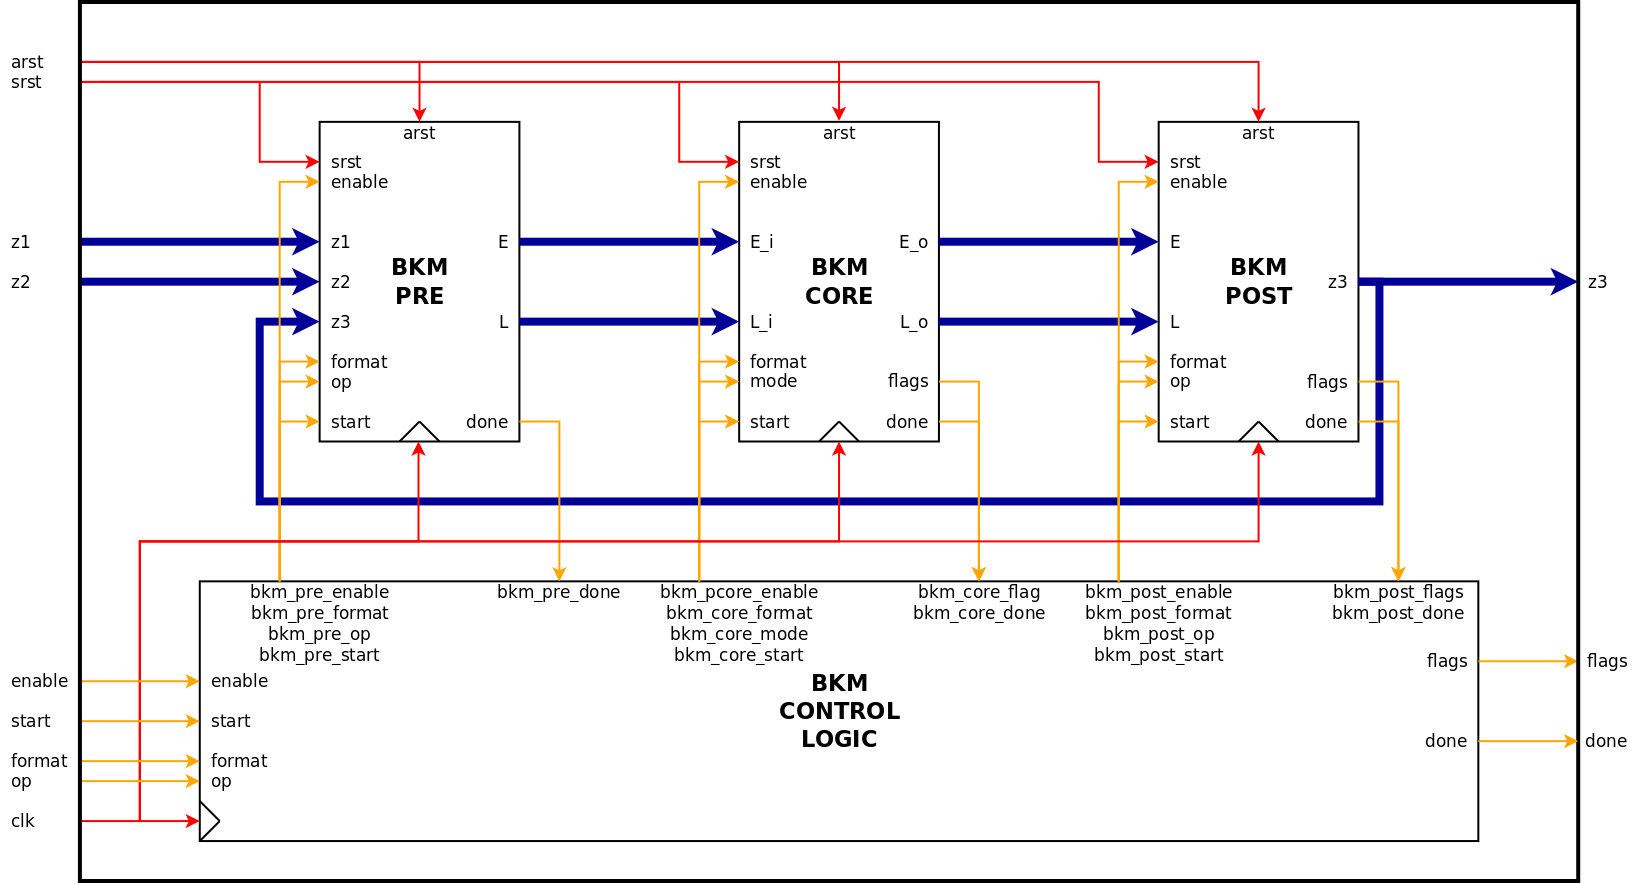
\includegraphics[width=1.0\textwidth]{./figures/bkm_fixed.png}
         \caption{Arquitecture del bloque BKM fixed.}
         \label{fig:bkm_fixed}
      \end{figure}

      \begin{table}[h]
      \centering
      \begin{tabular}{lccl}
         \hline
         Puerto            &  Tama\~no    &  Direcci\'on    &  Descripci\'on                                                  \\ \hline \hline
         \verb|clk      |  &  1  bit      &  Input          &  Clock signal                                                   \\ \hline
         \verb|arst     |  &  1   bit      &  Input          &  Active high asynchronous reset signal                          \\ \hline
         \verb|srst     |  &  1  bit      &  Input          &  Active high synchronous reset signal                           \\ \hline
         \verb|enable   |  &  1  bit      &  Input          &  Active high enable signal                                      \\ \hline
         \verb|start    |  &  1  bit      &  Input          &  Active high start signal                                       \\ \hline
         \verb|format   |  &  2  bit      &  Input          &  Format specifier (0/1): MSB for complex/real, LSB for 64/32 bits\\ \hline
         \verb|op       |  &  5  bits     &  Input          &  Operation code                                                 \\ \hline
         \verb|x_1      |  &  64 bits     &  Input          &  Real      part of input variable z1                            \\ \hline
         \verb|y_1      |  &  64 bits     &  Input          &  Imaginary part of input variable z1                            \\ \hline
         \verb|x_2      |  &  64 bits     &  Input          &  Real      part of input variable z2                            \\ \hline
         \verb|y_2      |  &  64 bits     &  Input          &  Imaginary part of input variable z2                            \\ \hline
         \verb|x_3      |  &  64 bits     &  Output         &  Real      part of output variable z3                           \\ \hline
         \verb|y_3      |  &  64 bits     &  Output         &  Imaginary part of output variable z3                           \\ \hline
         \verb|flags    |  &  1  bit      &  Output         &  Active high invert output signal                               \\ \hline
         \verb|done     |  &  1  bit      &  Output         &  Active high done signal: Stays asserted until start strobe     \\ \hline
      \end{tabular}
      \caption{Puertos del bloque op decoder.}
      \label{tab:bkm_fixed_ports}
      \end{table}


      \subsection{BKM Pre}
      Este bloque se encarga de 
      \begin{table}[h]
      \centering
      \begin{tabular}{lccl}
         \hline
         Puerto            &  Tama\~no    &  Direcci\'on    &  Descripci\'on                                                  \\ \hline \hline
         \verb|clk      |  &  1  bit      &  Input          &  Clock signal                                                   \\ \hline
         \verb|arst     |  &  1  bit      &  Input          &  Active high asynchronous reset signal                          \\ \hline
         \verb|srst     |  &  1  bit      &  Input          &  Active high synchronous reset signal                           \\ \hline
         \verb|enable   |  &  1  bit      &  Input          &  Active high enable signal                                      \\ \hline
         \verb|start    |  &  1  bit      &  Input          &  Active high start signal                                       \\ \hline
         \verb|format   |  &  2  bit      &  Input          &  Format specifier (0/1): MSB for complex/real, LSB for 64/32 bits\\ \hline
         \verb|op       |  &  5  bits     &  Input          &  Operation code                                                 \\ \hline
         \verb|x_1      |  &  64 bits     &  Input          &  Real      part of input variable z1                            \\ \hline
         \verb|y_1      |  &  64 bits     &  Input          &  Imaginary part of input variable z1                            \\ \hline
         \verb|x_2      |  &  64 bits     &  Input          &  Real      part of input variable z2                            \\ \hline
         \verb|y_2      |  &  64 bits     &  Input          &  Imaginary part of input variable z2                            \\ \hline
         \verb|x_3      |  &  64 bits     &  Output         &  Real      part of output variable z3                           \\ \hline
         \verb|y_3      |  &  64 bits     &  Output         &  Imaginary part of output variable z3                           \\ \hline
         \verb|flags    |  &  1  bit      &  Output         &  Active high invert output signal                               \\ \hline
         \verb|done     |  &  1  bit      &  Output         &  Active high done signal: Stays asserted until start strobe     \\ \hline
      \end{tabular}
      \caption{Puertos del bloque op decoder.}
      \label{tab:bkm_fixed_ports}
      \end{table}
      \subsection{BKM Post}
      \subsection{BKM Fixed control logic}


   \section{BKM Core}


\end{document}






